% Gabarit pandoc des corrigés publiés (brut et guidé). Contenu sans marque ni nom de site.
% Compilation : lualatex (latexmk -lualatex).
% Le Markdown reste la source unique : ne pas éditer ce fichier .tex à la main.
\documentclass[11pt,a4paper]{article}

% --- Moteur, polices (Latin Modern) et langue ---------------------------------
\usepackage{iftex}
\ifLuaTeX\else\errmessage{Ce document se compile avec lualatex}\fi
\usepackage{amsmath,amssymb,mathtools}
\usepackage{fontspec}
% mathrm=sym : \mathrm prend ses glyphes dans la police mathématique (ℓ, μ, Ω), comme KaTeX.
\usepackage[math-style=TeX,bold-style=TeX,mathrm=sym]{unicode-math}
% Repli pour les glyphes absents de Latin Modern (indices et exposants Unicode,
% flèches, filets des schémas en texte, symboles) : DejaVu, puis Latin Modern Math
% (ℓ, lettres mathématiques Unicode des légendes).
\directlua{
  luaotfload.add_fallback("repliTexte", {"DejaVuSerif:mode=harf;", "DejaVuSans:mode=harf;", "file:latinmodern-math.otf:mode=harf;"})
  luaotfload.add_fallback("repliMono", {"DejaVuSansMono:mode=harf;", "DejaVuSans:mode=harf;", "file:latinmodern-math.otf:mode=harf;"})
}
\setmainfont{Latin Modern Roman}[RawFeature={fallback=repliTexte}]
\setsansfont{Latin Modern Sans}[RawFeature={fallback=repliTexte}]
\setmonofont{Latin Modern Mono}[RawFeature={fallback=repliMono}]
\setmathfont{Latin Modern Math}
\usepackage[french]{babel}
\frenchsetup{SmallCapsFigTabCaptions=false}

% --- Mise en page --------------------------------------------------------------
\usepackage[a4paper,margin=2.2cm,headheight=14pt,footskip=1.2cm]{geometry}
\usepackage{microtype}
\setlength{\emergencystretch}{4em}
\tolerance=1500
\setlength{\parindent}{0pt}
\setlength{\parskip}{0.55\baselineskip plus 2pt minus 1pt}
\usepackage{xcolor}
% Gris nommés : babel-french rend « ! » actif dans le document.
\definecolor{gris2}{gray}{0.98}
\definecolor{gris3}{gray}{0.97}
\definecolor{gris5}{gray}{0.95}
\definecolor{gris35}{gray}{0.65}
\definecolor{gris40}{gray}{0.60}
\definecolor{gris45}{gray}{0.55}
\definecolor{gris50}{gray}{0.50}
\definecolor{gris55}{gray}{0.45}
\definecolor{gris60}{gray}{0.40}
\definecolor{gris65}{gray}{0.35}
\definecolor{gris70}{gray}{0.30}
\definecolor{gris80}{gray}{0.20}
\definecolor{gris85}{gray}{0.15}
\usepackage{graphicx}
\usepackage{float}
\usepackage{caption}
\captionsetup{font=small,labelformat=empty,justification=centering}
\usepackage{booktabs,longtable,array,multirow,calc}
\usepackage{siunitx}
\sisetup{locale=FR}
\usepackage[version=4]{mhchem}
\usepackage{listings}
\usepackage{fancyhdr}
\usepackage{lastpage}
\usepackage[most]{tcolorbox}
\usepackage{enumitem}
\setlist{nosep,leftmargin=*,topsep=2pt}
\usepackage[hidelinks,unicode]{hyperref}
\usepackage{bookmark}
\hypersetup{pdftitle={Banque PT — Mathématiques C 2026},pdfauthor={Rédigé par IA},pdfcreator={LaTeX},pdfsubject={Corrigé brut}}
\usepackage{xurl}

% --- Pandoc : listes, tableaux, figures ----------------------------------------
\providecommand{\passthrough}[1]{#1}
\providecommand{\tightlist}{\setlength{\itemsep}{0pt}\setlength{\parskip}{0pt}}

\makeatletter
\def\maxwidth{\ifdim\Gin@nat@width>\linewidth\linewidth\else\Gin@nat@width\fi}
\def\maxheight{\ifdim\Gin@nat@height>0.55\textheight 0.55\textheight\else\Gin@nat@height\fi}
\makeatother
\setkeys{Gin}{width=\maxwidth,height=\maxheight,keepaspectratio}
\setcounter{secnumdepth}{-\maxdimen}
\providecommand{\pandocbounded}[1]{#1}
\usepackage{longtable,booktabs,array}

% --- Code (listings) -----------------------------------------------------------
\lstset{
  basicstyle=\ttfamily\small,
  columns=fullflexible,
  keepspaces=true,
  breaklines=true,
  breakatwhitespace=false,
  postbreak=\mbox{\textcolor{gris50}{$\hookrightarrow$}\space},
  frame=single,
  rulecolor=\color{gris35},
  framesep=4pt,
  xleftmargin=5pt,xrightmargin=5pt,
  backgroundcolor=\color{gris3},
  keywordstyle=\bfseries,
  commentstyle=\color{gris65},
  stringstyle=\color{gris80},
  showstringspaces=false,
  tabsize=4,
  extendedchars=true,
  aboveskip=6pt,belowskip=6pt,
}

% --- Macros des corrigés (KaTeX ↔ LaTeX) ---------------------------------------
% Les corrigés sont écrits pour KaTeX : on définit ici ce que KaTeX connaît et
% que LaTeX n'a pas, sans jamais retoucher le Markdown.
\providecommand{\R}{\mathbb{R}}
\providecommand{\N}{\mathbb{N}}
\providecommand{\Z}{\mathbb{Z}}
\providecommand{\Q}{\mathbb{Q}}
\providecommand{\C}{\mathbb{C}}
\providecommand{\dd}{\mathrm{d}}
\providecommand{\llbracket}{\lBrack}
\providecommand{\rrbracket}{\rBrack}
\providecommand{\lBrace}{\lbrace}
\providecommand{\rBrace}{\rbrace}
\providecommand{\Box}{\square}
\providecommand{\Diamond}{\lozenge}
\providecommand{\varnothing}{\emptyset}
\providecommand{\argmax}{\operatorname*{arg\,max}}
\providecommand{\argmin}{\operatorname*{arg\,min}}
\renewcommand{\leq}{\leqslant}
\renewcommand{\geq}{\geqslant}

% Équation hors texte : réduite à la largeur de la ligne si elle déborde.
\newsavebox{\boiteequation}
\newcommand{\equationajustee}[1]{%
  \sbox{\boiteequation}{$\displaystyle #1$}%
  \ifdim\wd\boiteequation>\linewidth
    \[\resizebox{\linewidth}{!}{\usebox{\boiteequation}}\]%
  \else
    \[#1\]%
  \fi}

% --- Encadrés pédagogiques (sobres, lisibles en noir et blanc) -----------------
\tcbset{
  encadre/.style={
    enhanced,breakable,sharp corners,
    colback=white,colframe=gris55,
    boxrule=0.4pt,leftrule=2.2pt,
    left=6pt,right=6pt,top=3pt,bottom=3pt,
    before skip=6pt,after skip=6pt,
    fonttitle=\bfseries\small,coltitle=black,
    attach title to upper,after title={\quad},
    parbox=false,
  }
}
\newtcolorbox{indication}[1]{encadre,colframe=gris45,colback=gris2,title={Indication~#1}}
\newtcolorbox{methode}{encadre,colframe=gris70,title={Méthode}}
\newtcolorbox{piege}{encadre,colframe=gris85,boxrule=0.8pt,leftrule=2.2pt,title={Piège}}
\newtcolorbox{jury}{encadre,colframe=gris60,colback=gris5,title={Jury}}
\newtcolorbox{encadrenote}{encadre,colframe=gris40}

% --- Titres de section ---------------------------------------------------------
\usepackage{titlesec}
\titleformat{\section}{\Large\bfseries}{}{0pt}{}
\titleformat{\subsection}{\large\bfseries}{}{0pt}{}
\titleformat{\subsubsection}{\normalsize\bfseries}{}{0pt}{}
\titlespacing*{\section}{0pt}{14pt plus 4pt minus 2pt}{6pt}
\titlespacing*{\subsection}{0pt}{10pt plus 3pt minus 2pt}{4pt}
\titlespacing*{\subsubsection}{0pt}{8pt plus 2pt minus 2pt}{2pt}

% --- En-tête et pied de page ---------------------------------------------------
\pagestyle{fancy}
\fancyhf{}
\fancyhead[L]{\small\textsc{Corrigé brut} · Banque PT PT}
\fancyhead[R]{\small Maths C 2026}
\fancyfoot[L]{\footnotesize Corrigé rédigé par IA, non officiel}
\fancyfoot[R]{\footnotesize \thepage\,/\,\pageref*{LastPage}}
\renewcommand{\headrulewidth}{0.4pt}
\renewcommand{\footrulewidth}{0pt}
\fancypagestyle{plain}{\fancyhf{}\fancyfoot[R]{\footnotesize \thepage\,/\,\pageref*{LastPage}}\fancyfoot[L]{\footnotesize Corrigé rédigé par IA, non officiel}\renewcommand{\headrulewidth}{0pt}}

\begin{document}
\thispagestyle{plain}
\begin{center}
  {\small\scshape Corrigé brut}\par\smallskip
  {\LARGE\bfseries Banque PT — Mathématiques C 2026\par}\medskip
  {\large Banque PT · PT · Maths C · 2026\par}
\end{center}
\vspace{2pt}\hrule\vspace{8pt}

\emph{Corrigé rédigé par IA, non officiel. Signalez toute erreur.}

Épreuve de 4 h, calculatrice interdite, une feuille de papier millimétré à rendre avec la copie.

\hypertarget{pruxe9ambule}{%
\section{Préambule}\label{pruxe9ambule}}

Dans tout le préambule, \(t_0>0\), et pour \(t\neq t_0\) :

\equationajustee{\begin{aligned}
f(t)&=\frac{t}{t_0-t},\\
g(t)&=\frac{t_0}{t_0-t}.
\end{aligned}}

\hypertarget{question-1}{%
\subsection{Question 1}\label{question-1}}

Les fonctions \(f\) et \(g\) sont des fonctions rationnelles. Leur dénominateur \(t_0-t\) ne s'annule pas sur \(\mathbb{R}\setminus\{t_0\}\). Elles sont donc dérivables sur

\equationajustee{\boxed{D=\mathbb{R}\setminus\{t_0\}=\,]-\infty,t_0[\,\cup\,]t_0,+\infty[}}

Pour \(t\in D\), on écrit le numérateur de \(f\) sous la forme \((t-t_0)+t_0\) :

\equationajustee{\begin{aligned}
f(t)&=\frac{(t-t_0)+t_0}{t_0-t}\\
&=-1+\frac{t_0}{t_0-t}\\
&=g(t)-1.
\end{aligned}}

Les fonctions \(f\) et \(g\) diffèrent d'une constante, donc \(f'=g'\) sur \(D\).

La dérivée de \(t\mapsto(t_0-t)^{-1}\) est \(t\mapsto(t_0-t)^{-2}\). Ainsi, pour tout \(t\in D\) :

\equationajustee{\boxed{\begin{aligned}
f'(t)&=g'(t)\\
&=\frac{t_0}{(t_0-t)^2}
\end{aligned}}}

\hypertarget{question-2}{%
\subsection{Question 2}\label{question-2}}

Pour \(t\in D\), \(f'(t)=\dfrac{t_0}{(t_0-t)^2}>0\) car \(t_0>0\).

La fonction \(f\) est donc strictement croissante sur \(]-\infty,t_0[\) et sur \(]t_0,+\infty[\), séparément : \(D\) n'est pas un intervalle.

Limites :
- en \(\pm\infty\) : pour \(t\neq0\), \(f(t)=\dfrac{1}{\frac{t_0}{t}-1}\), qui tend vers \(-1\) ;
- en \(t_0^-\) : le numérateur tend vers \(t_0>0\) et \(t_0-t\to0^+\), donc \(f(t)\to+\infty\) ;
- en \(t_0^+\) : le numérateur tend vers \(t_0>0\) et \(t_0-t\to0^-\), donc \(f(t)\to-\infty\).

\begin{longtable}[]{@{}llllll@{}}
\toprule\noalign{}
\(t\) & \(-\infty\) & & \(t_0^-\) ‖ \(t_0^+\) & & \(+\infty\) \\
\midrule\noalign{}
\endhead
\bottomrule\noalign{}
\endlastfoot
\(f'(t)\) & & \(+\) & ‖ & \(+\) & \\
\(f(t)\) & −1 & ↗ & +∞ ‖ −∞ & ↗ & −1 \\
\end{longtable}

Les droites \(t=t_0\) et \(y=-1\) sont asymptotes à la courbe.

\hypertarget{question-3}{%
\subsection{Question 3}\label{question-3}}

On a \(f(0)=0\) et \(f'(0)=\dfrac{t_0}{t_0^2}=\dfrac1{t_0}\). La tangente en \(0\) a pour équation \(y=f(0)+f'(0)(t-0)\), soit

\equationajustee{\boxed{T:\ y=\frac{t}{t_0}}}

\hypertarget{question-4}{%
\subsection{Question 4}\label{question-4}}

Pour \(t_0=1\), \(f(t)=\dfrac{t}{1-t}\). La tangente en \(0\) est \(T:y=t\). L'asymptote verticale est \(t=1\), l'asymptote horizontale \(y=-1\).

Position relative :

\equationajustee{\begin{aligned}
f(t)-t&=\frac{t-t(1-t)}{1-t}\\
&=\frac{t^2}{1-t}.
\end{aligned}}

La courbe est donc \textbf{au-dessus de \(T\) pour \(t<1\)} (elle la touche seulement en \(0\)), et \textbf{au-dessous de \(T\) pour \(t>1\)}.

Valeurs utiles pour le tracé (1 cm par unité) :

\begin{longtable}[]{@{}
  >{\raggedright\arraybackslash}p{(\columnwidth - 24\tabcolsep) * \real{0.0769}}
  >{\raggedright\arraybackslash}p{(\columnwidth - 24\tabcolsep) * \real{0.0769}}
  >{\raggedright\arraybackslash}p{(\columnwidth - 24\tabcolsep) * \real{0.0769}}
  >{\raggedright\arraybackslash}p{(\columnwidth - 24\tabcolsep) * \real{0.0769}}
  >{\raggedright\arraybackslash}p{(\columnwidth - 24\tabcolsep) * \real{0.0769}}
  >{\raggedright\arraybackslash}p{(\columnwidth - 24\tabcolsep) * \real{0.0769}}
  >{\raggedright\arraybackslash}p{(\columnwidth - 24\tabcolsep) * \real{0.0769}}
  >{\raggedright\arraybackslash}p{(\columnwidth - 24\tabcolsep) * \real{0.0769}}
  >{\raggedright\arraybackslash}p{(\columnwidth - 24\tabcolsep) * \real{0.0769}}
  >{\raggedright\arraybackslash}p{(\columnwidth - 24\tabcolsep) * \real{0.0769}}
  >{\raggedright\arraybackslash}p{(\columnwidth - 24\tabcolsep) * \real{0.0769}}
  >{\raggedright\arraybackslash}p{(\columnwidth - 24\tabcolsep) * \real{0.0769}}
  >{\raggedright\arraybackslash}p{(\columnwidth - 24\tabcolsep) * \real{0.0769}}@{}}
\toprule\noalign{}
\begin{minipage}[b]{\linewidth}\raggedright
t
\end{minipage} & \begin{minipage}[b]{\linewidth}\raggedright
−4
\end{minipage} & \begin{minipage}[b]{\linewidth}\raggedright
−2
\end{minipage} & \begin{minipage}[b]{\linewidth}\raggedright
−1
\end{minipage} & \begin{minipage}[b]{\linewidth}\raggedright
0
\end{minipage} & \begin{minipage}[b]{\linewidth}\raggedright
0,5
\end{minipage} & \begin{minipage}[b]{\linewidth}\raggedright
0,75
\end{minipage} & \begin{minipage}[b]{\linewidth}\raggedright
0,9
\end{minipage} & \begin{minipage}[b]{\linewidth}\raggedright
1,1
\end{minipage} & \begin{minipage}[b]{\linewidth}\raggedright
1,5
\end{minipage} & \begin{minipage}[b]{\linewidth}\raggedright
2
\end{minipage} & \begin{minipage}[b]{\linewidth}\raggedright
3
\end{minipage} & \begin{minipage}[b]{\linewidth}\raggedright
5
\end{minipage} \\
\midrule\noalign{}
\endhead
\bottomrule\noalign{}
\endlastfoot
f(t) & −0,8 & −0,67 & −0,5 & 0 & 1 & 3 & 9 & −11 & −3 & −2 & −1,5 & −1,25 \\
\end{longtable}

\begin{figure}[H]
\centering
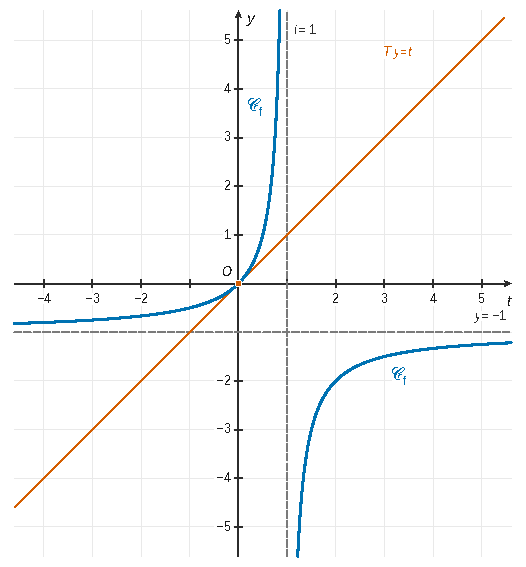
\includegraphics{figures/preambule-q4-trace-f.pdf}
\caption*{Figure 1 --- Courbe de f(t) = t/(1 − t) (t₀ = 1), tangente T : y = t en
O, asymptotes t = 1 et y = −1}
\end{figure}

La figure est réduite ; sur la copie, on trace à 1 cm par unité, et la tangente, les deux asymptotes et la courbe figurent sur le même graphique.

La branche gauche (\(t<1\)) rejoint \(y=-1\) par au-dessus en \(-\infty\). La branche droite (\(t>1\)) la rejoint par en dessous, car \(f(t)+1=\dfrac{1}{1-t}<0\). La droite \(T\) ne rencontre la courbe qu'en l'origine.

La courbe est symétrique par rapport au centre \((1,-1)\), intersection des asymptotes : c'est une hyperbole.

\hypertarget{question-5}{%
\subsection{Question 5}\label{question-5}}

Comme \(f=g-1\), il suffit de dériver \(g\). Montrons par récurrence sur \(n\ge1\) la propriété \(({\mathcal{H}}_n)\) :

« \(g\) est \(n\) fois dérivable sur \(D\) et, pour tout \(t\in D\), \(g^{(n)}(t)=\dfrac{n!\,t_0}{(t_0-t)^{n+1}}\) ».

\begin{itemize}
\tightlist
\item
  \textbf{Initialisation} : \(({\mathcal{H}}_1)\) est la question 1.
\item
  \textbf{Hérédité} : supposons \(({\mathcal{H}}_n)\).
\end{itemize}

La fonction \(t\mapsto n!\,t_0\,(t_0-t)^{-(n+1)}\) est dérivable sur \(D\), comme composée de fonctions dérivables (une fonction affine, puis une puissance entière négative sur \({\mathbb{R}}^*\)). Donc \(g\) est \((n+1)\) fois dérivable sur \(D\), et

\equationajustee{\begin{aligned}
g^{(n+1)}(t)&=n!\,t_0\cdot\big(-(n+1)\big)(t_0-t)^{-(n+2)}\cdot(-1)\\
&=\frac{(n+1)!\,t_0}{(t_0-t)^{n+2}}.
\end{aligned}}

C'est \(({\mathcal{H}}_{n+1})\).

Ainsi \(f\) est \(n\) fois dérivable sur \(]-\infty,t_0[\) et sur \(]t_0,+\infty[\), et pour \(n\ge1\) et \(t\neq t_0\) :

\equationajustee{\boxed{f^{(n)}(t)=\frac{n!\,t_0}{(t_0-t)^{n+1}}}}

\hypertarget{question-6}{%
\subsection{Question 6}\label{question-6}}

Sur chacun des intervalles \(]-\infty,t_0[\) et \(]t_0,+\infty[\), la fonction \(t\mapsto -t_0\ln|t_0-t|\) est dérivable. Sa dérivée vaut \(-t_0\cdot\dfrac{-1}{t_0-t}=g(t)\). La valeur absolue est nécessaire : sur \(]t_0,+\infty[\), \(t_0-t<0\).

Comme \(f=-1+g\), il suffit d'ajouter une primitive de la constante \(-1\). Sur chacun des deux intervalles :

\equationajustee{\boxed{G(t)=-t_0\ln|t_0-t|}}

\equationajustee{\boxed{F(t)=-t-t_0\ln|t_0-t|}}

Ces primitives sont valables sur chacun des deux intervalles, à une constante additive près sur chacun.

\hypertarget{question-7}{%
\subsection{Question 7}\label{question-7}}

\textbf{Formule de Taylor-Young.} Soit \(n\in{\mathbb{N}}^*\), \(I\) un intervalle de \(\mathbb{R}\) et \(x_0\in I\).

Soit \(\psi\) de classe \({\mathcal{C}}^n\) sur \(I\).

Alors, quand \(x\to x_0\) avec \(x\in I\) :

\equationajustee{\boxed{\psi(x)=\sum_{k=0}^{n}\frac{\psi^{(k)}(x_0)}{k!}(x-x_0)^k+o\big((x-x_0)^n\big)}}

De façon équivalente, quand \(h\to0\) avec \(x_0+h\in I\) :

\equationajustee{\psi(x_0+h)=\sum_{k=0}^{n}\frac{\psi^{(k)}(x_0)}{k!}h^k+o(h^n).}

\hypertarget{question-8}{%
\subsection{Question 8}\label{question-8}}

La fonction \(t\mapsto\dfrac1{1-t}\) est définie sur \(\boxed{\mathbb{R}\setminus\{1\}}\). C'est la fonction \(g\) du préambule pour \(t_0=1\).

Elle est de classe \({\mathcal{C}}^\infty\) sur l'intervalle \(I=\,]-\infty,1[\), qui contient \(0\).

On calcule ses dérivées en \(0\) pour \(0\le k\le n\). On a \(g(0)=1\), et la question 5 donne, pour \(k\ge1\) :

\equationajustee{g^{(k)}(0)=\frac{k!\cdot1}{(1-0)^{k+1}}=k!.}

Ainsi \(\dfrac{g^{(k)}(0)}{k!}=1\) pour tout \(k\in\{0,\dots,n\}\). La formule de Taylor-Young à l'ordre \(n\) en \(0\) (question 7, sur \(I\)) donne, quand \(t\to0\) :

\equationajustee{\boxed{\begin{aligned}
\frac1{1-t}&=\sum_{k=0}^n t^k+o(t^n)\\
&=1+t+t^2+\cdots+t^n+o(t^n)
\end{aligned}}}

Vérification directe :

\equationajustee{\begin{aligned}
\frac1{1-t}-\sum_{k=0}^nt^k&=\frac{t^{n+1}}{1-t}\\
&=t^n\cdot\frac{t}{1-t},
\end{aligned}}

et \(\dfrac{t}{1-t}\to0\) quand \(t\to0\).

\hypertarget{question-9}{%
\subsection{Question 9}\label{question-9}}

La fonction \(\ell:t\mapsto\ln(1-t)\) est définie sur \(\boxed{]-\infty,1[}\), puisqu'il faut \(1-t>0\). Elle y est de classe \({\mathcal{C}}^\infty\), et \(\ell'(t)=-\dfrac1{1-t}\).

\textbf{DL de \(\ell'\) à l'ordre \(n-1\).} Pour \(n\ge2\), la question 8 à l'ordre \(n-1\) donne

\equationajustee{\ell'(t)=-\sum_{k=0}^{n-1}t^k+o(t^{n-1}).}

Pour \(n=1\), c'est \(\ell'(t)=-1+o(1)\), par continuité de \(\ell'\) en \(0\).

\textbf{Théorème d'intégration des développements limités.} Soit \(\ell\) dérivable sur un intervalle contenant \(0\), telle que \(\ell'\) admette en \(0\) un développement limité à l'ordre \(n-1\).

Alors \(\ell\) admet en \(0\) un développement limité à l'ordre \(n\). On l'obtient en primitivant terme à terme la partie régulière, la constante étant \(\ell(0)\).

Ici \(\ell(0)=\ln1=0\), d'où

\equationajustee{\ell(t)=\ell(0)-\sum_{k=0}^{n-1}\frac{t^{k+1}}{k+1}+o(t^n),}

soit, quand \(t\to0\) :

\equationajustee{\boxed{\begin{aligned}
\ln(1-t)&=-\sum_{k=1}^n\frac{t^k}{k}+o(t^n)\\
&=-t-\frac{t^2}{2}-\cdots-\frac{t^n}{n}+o(t^n)
\end{aligned}}}

On peut aussi appliquer directement Taylor-Young à \(\ell\). Pour \(k\ge1\), \(\ell^{(k)}=-g^{(k-1)}\) avec \(t_0=1\). D'où \(\ell^{(k)}(0)=-(k-1)!\) et \(\dfrac{\ell^{(k)}(0)}{k!}=-\dfrac1k\).

\hypertarget{partie-i}{%
\section{Partie I}\label{partie-i}}

\hypertarget{question-1-1}{%
\subsection{Question 1}\label{question-1-1}}

Pour \(t>0\), comme \((1+t)-t=1\) :

\equationajustee{h(t)=\frac1{t(1+t)}=\frac1t-\frac1{1+t}.}

Une primitive de \(h\) sur \({\mathbb{R}}_+^*\) est donc

\equationajustee{\boxed{H(t)=\ln\frac{t}{1+t}}}

\hypertarget{question-2-1}{%
\subsection{Question 2}\label{question-2-1}}

Soit \(n\ge2\). La fonction \(h\) est continue et positive sur \([n,+\infty[\), et \(h(t)\underset{+\infty}{\sim}\dfrac1{t^2}\).

L'intégrale de Riemann \(\int_1^{+\infty}\frac{dt}{t^2}\) converge (\(2>1\)). Par le théorème de comparaison des intégrales de fonctions positives, l'intégrale \(\int_n^{+\infty}h\) \textbf{converge}.

Pour \(A>n\) :

\equationajustee{\int_n^A h=H(A)-H(n)=\ln\frac{A}{1+A}-\ln\frac{n}{n+1}.}

Or \(\ln\frac{A}{1+A}\to\ln1=0\) quand \(A\to+\infty\). Donc

\equationajustee{\boxed{\int_n^{+\infty}\frac{dt}{t+t^2}=\ln\Big(1+\frac1n\Big)}}

\hypertarget{question-3-1}{%
\subsection{Question 3}\label{question-3-1}}

Soit \(n\ge2\). Pour tout réel \(t\), \(n+\cos(nt)\ge n-1\ge1>0\).

La fonction \(t\mapsto\ln\big(n+\cos(nt)\big)\) est donc définie et dérivable sur \([0,\pi]\), de dérivée \(\dfrac{-n\sin(nt)}{n+\cos(nt)}\). Par suite, avec \(\cos(n\pi)=(-1)^n\) :

\equationajustee{\begin{aligned}
-n\int_0^\pi\frac{\sin(nt)}{n+\cos(nt)}\,dt&=\Big[\ln\big(n+\cos(nt)\big)\Big]_0^\pi\\
&=\ln\big(n+\cos(n\pi)\big)-\ln(n+1)\\
&=\ln\frac{n+(-1)^n}{n+1}.
\end{aligned}}

Avec la question 2 :

\equationajustee{\begin{aligned}
u_n&=\ln\frac{n+(-1)^n}{n+1}+\ln\frac{n+1}{n}\\
&=\ln\frac{n+(-1)^n}{n},
\end{aligned}}

soit, pour \(n\ge2\) :

\equationajustee{\boxed{u_n=\ln\Big(1+\frac{(-1)^n}{n}\Big)}}

\hypertarget{question-4-1}{%
\subsection{Question 4}\label{question-4-1}}

On a \(\dfrac{(-1)^n}{n}\to0\) et \(\ln\) est continue en \(1\). Par composition des limites :

\equationajustee{\boxed{\lim_{n\to+\infty}u_n=0}}

\hypertarget{question-5-1}{%
\subsection{Question 5}\label{question-5-1}}

Notons, à partir d'un même indice initial \(n_0\), les sommes partielles

\equationajustee{\begin{aligned}
A_N&=\sum_{k=n_0}^N a_k,\\
B_N&=\sum_{k=n_0}^N b_k.
\end{aligned}}

Par hypothèse, elles convergent vers des réels \(A\) et \(B\). Par linéarité des sommes finies :

\equationajustee{\sum_{k=n_0}^N(a_k+\lambda b_k)=A_N+\lambda B_N.}

Le membre de droite converge vers \(A+\lambda B\) quand \(N\to+\infty\), par opérations sur les limites. La suite des sommes partielles de \(\sum(a_n+\lambda b_n)\) converge donc :

\equationajustee{\boxed{\sum(a_n+\lambda b_n)\ \text{converge, de somme}\ \sum_{n=n_0}^{+\infty} a_n+\lambda\sum_{n=n_0}^{+\infty} b_n}}

\hypertarget{question-6-1}{%
\subsection{Question 6}\label{question-6-1}}

On pose \(h=\frac1n\to0\). La question 9 du préambule, avec \(t=-x\), donne \(\ln(1+x)=x-\dfrac{x^2}2+o(x^2)\) quand \(x\to0\). Avec \(x=(-1)^nh\), on a \(x^2=h^2\) et

\equationajustee{\begin{aligned}
u_n&=(-1)^nh-\frac{h^2}{2}+o(h^2)\\
&=\frac{(-1)^n}{n}-\frac1{2n^2}+o\Big(\frac1{n^2}\Big).
\end{aligned}}

Posons \(a_n=\dfrac{(-1)^n}{n}\) et \(b_n=u_n-a_n\). On a \(b_n\sim-\dfrac1{2n^2}\).

\begin{itemize}
\tightlist
\item
  \(\sum a_n\) converge par le critère spécial des séries alternées : la suite \(\big(\frac1n\big)\) est positive, décroissante et tend vers \(0\).
\item
  \(\sum b_n\) converge absolument : \(|b_n|\sim\dfrac1{2n^2}\), terme d'une série de Riemann convergente (comparaison de séries à termes positifs).
\item
  Par la question 5 avec \(\lambda=1\), \(\sum u_n=\sum(a_n+b_n)\) \textbf{converge}.
\end{itemize}

Convergence absolue : \(|u_n|=\Big|\frac{(-1)^n}{n}+b_n\Big|\) avec \(b_n=o(1/n)\), donc \(|u_n|\sim\dfrac1n\). La série harmonique diverge. Par comparaison de séries à termes positifs, \(\sum|u_n|\) \textbf{diverge}.

\equationajustee{\boxed{\sum_{n\ge2}u_n\ \text{converge mais ne converge pas absolument}}}

\hypertarget{question-7-1}{%
\subsection{Question 7}\label{question-7-1}}

D'après la question 3 :
- pour \(n\) pair, \(u_n=\ln\dfrac{n+1}{n}\) ;
- pour \(n\) impair, \(u_n=\ln\dfrac{n-1}{n}\).

\textbf{(a)} Récurrence sur \(N\ge1\).

Pour \(N=1\) : \(S_2=u_2=\ln\frac32=\ln\frac{2\cdot1+1}{2\cdot1}\).

Si \(S_{2N}=\ln\dfrac{2N+1}{2N}\), alors

\equationajustee{\begin{aligned}
S_{2N+2}&=S_{2N}+u_{2N+1}+u_{2N+2}\\
&=\ln\frac{2N+1}{2N}+\ln\frac{2N}{2N+1}+\ln\frac{2N+3}{2N+2}\\
&=\ln\frac{2N+3}{2N+2}.
\end{aligned}}

Donc, pour tout \(N\ge1\) :

\equationajustee{\boxed{S_{2N}=\ln\frac{2N+1}{2N}}}

On peut aussi séparer les indices pairs et impairs :

\equationajustee{\begin{aligned}
S_{2N}&=\sum_{k=1}^{N}u_{2k}+\sum_{k=1}^{N-1}u_{2k+1}\\
&=\sum_{k=1}^{N}\big(\ln(2k+1)-\ln(2k)\big)+\sum_{k=1}^{N-1}\big(\ln(2k)-\ln(2k+1)\big)\\
&=\ln(2N+1)-\ln(2N).
\end{aligned}}

\textbf{(b)} Pour \(n\ge1\) :

\equationajustee{\begin{aligned}
u_{2n}&=\ln\frac{2n+1}{2n}>0,\\
u_{2n+1}&=\ln\frac{2n}{2n+1}=-\ln\frac{2n+1}{2n}.
\end{aligned}}

Les deux termes sont opposés :

\equationajustee{\boxed{u_{2n+1}=-u_{2n}}}

\textbf{(c)} Soit \(N\ge2\). Les indices \(2,\dots,2N-1\) se regroupent en \(N-1\) paires \((2n,2n+1)\), pour \(1\le n\le N-1\). Par (b) :

\equationajustee{\begin{aligned}
S_{2N-1}&=\sum_{n=1}^{N-1}(u_{2n}+u_{2n+1})\\
&=0.
\end{aligned}}

\equationajustee{\boxed{S_{2N-1}=0\quad(N\ge2)}}

Vérification avec (a) :

\equationajustee{\begin{aligned}
S_{2N-1}&=S_{2N}-u_{2N}\\
&=\ln\frac{2N+1}{2N}-\ln\frac{2N+1}{2N}\\
&=0.
\end{aligned}}

\textbf{(d)} On a \(S_{2N}=\ln\Big(1+\dfrac1{2N}\Big)\to0\) et \(S_{2N-1}=0\). Les suites extraites d'indices pairs et impairs de \((S_N)\) convergent vers la même limite \(0\), donc \((S_N)\) converge vers \(0\) :

\equationajustee{\boxed{\sum_{n=2}^{+\infty}u_n=0}}

\hypertarget{partie-ii}{%
\section{Partie II}\label{partie-ii}}

Pour \(n\ge1\) et \(x>1\), avec \(\ln x>0\) :

\equationajustee{G_n(x)=\int_0^{+\infty}x^{-nt}t^n\,dt=\int_0^{+\infty}t^ne^{-nt\ln x}\,dt.}

\hypertarget{question-1-2}{%
\subsection{Question 1}\label{question-1-2}}

Soit \(x>1\). La fonction \(\theta:t\mapsto t^ne^{-nt\ln x}\) est continue et positive sur \([0,+\infty[\). La borne \(0\) ne pose pas de problème : la seule borne impropre est \(+\infty\).

Comme \(n\ln x>0\), les croissances comparées donnent \(t^2\theta(t)=t^{n+2}e^{-nt\ln x}\to0\) quand \(t\to+\infty\). Donc \(\theta(t)=o\big(\frac1{t^2}\big)\) en \(+\infty\).

L'intégrale de Riemann \(\int_1^{+\infty}\frac{dt}{t^2}\) converge. Par le théorème de comparaison des intégrales de fonctions positives, \(\int_1^{+\infty}\theta\) converge, et \(\int_0^1\theta\) est l'intégrale d'une fonction continue sur un segment. Donc

\equationajustee{\boxed{G_n(x)\ \text{converge (absolument) pour tout}\ x>1}}

\hypertarget{question-2-2}{%
\subsection{Question 2}\label{question-2-2}}

Soit \(a>1\) et \(\Phi(x,t)=t^nx^{-nt}\) sur \([a,+\infty[\times[0,+\infty[\).
- Pour tout \(t\ge0\), \(x\mapsto\Phi(x,t)\) est continue sur \([a,+\infty[\).
- Pour tout \(x\ge a\), \(t\mapsto\Phi(x,t)\) est continue sur \([0,+\infty[\).
- Domination : pour \(x\ge a\) et \(t\ge0\), \(-nt\ln x\le-nt\ln a\), donc \(0\le\Phi(x,t)\le t^na^{-nt}\).
- Le majorant \(t\mapsto t^na^{-nt}\) est continu, positif et indépendant de \(x\). Il est intégrable sur \([0,+\infty[\) : son intégrale est \(G_n(a)\), convergente par la question 1.

Par le théorème de continuité des intégrales à paramètre :

\equationajustee{\boxed{G_n\ \text{est continue sur}\ [a,+\infty[}}

Ceci valant pour tout \(a>1\), \(G_n\) est continue sur \(]1,+\infty[\).

\hypertarget{question-3-2}{%
\subsection{Question 3}\label{question-3-2}}

Soit \(a>1\). Pour tout \(t\ge0\), \(x\mapsto\Phi(x,t)=t^ne^{-nt\ln x}\) est de classe \({\mathcal{C}}^1\) sur \([a,+\infty[\), et

\equationajustee{\frac{\partial\Phi}{\partial x}(x,t)=-n\,t^{n+1}x^{-nt-1}.}

Pour \(x\) fixé, cette dérivée est continue en \(t\). Pour \(x\ge a\) et \(t\ge0\), \(x^{-nt}\le a^{-nt}\) et \(x^{-1}\le a^{-1}\), d'où la domination

\equationajustee{\Big|\frac{\partial\Phi}{\partial x}(x,t)\Big|\le\psi_a(t),}

où l'on a posé

\equationajustee{\psi_a(t)=n\,t^{n+1}a^{-nt-1}.}

Le majorant \(\psi_a\) est indépendant de \(x\), continu et positif sur \([0,+\infty[\).

Il est intégrable : par croissances comparées, \(t^2\psi_a(t)\to0\) en \(+\infty\), donc \(\psi_a(t)=o(1/t^2)\), et l'intégrale de Riemann \(\int_1^{+\infty}\frac{dt}{t^2}\) converge.

Par le théorème de dérivation des intégrales à paramètre, \(G_n\) est de classe \({\mathcal{C}}^1\) sur \([a,+\infty[\), et pour \(x\ge a\) :

\equationajustee{\boxed{\begin{aligned}
G_n'(x)&=-n\int_0^{+\infty}t^{n+1}x^{-nt-1}\,dt\\
&=-\frac nx\int_0^{+\infty}t^{n+1}x^{-nt}\,dt
\end{aligned}}}

\hypertarget{question-4-2}{%
\subsection{Question 4}\label{question-4-2}}

Soit \(x>1\) et \(n\ge1\). Dans \(G_{n+1}(x)=\int_0^{+\infty}t^{n+1}x^{-(n+1)t}\,dt\), on pose \(u=\dfrac{(n+1)t}{n}\). C'est un changement de variable affine, bijectif de \([0,+\infty[\) sur lui-même, avec

\equationajustee{\begin{aligned}
t&=\frac{n}{n+1}u,\\
dt&=\frac{n}{n+1}\,du,\\
(n+1)t&=nu.
\end{aligned}}

Il vient

\equationajustee{G_{n+1}(x)=\Big(\frac{n}{n+1}\Big)^{n+2}\int_0^{+\infty}u^{n+1}x^{-nu}\,du.}

On intègre par parties sur \([0,A]\). On dérive \(u\mapsto u^{n+1}\) et on primitive \(u\mapsto x^{-nu}=e^{-nu\ln x}\) en \(u\mapsto-\dfrac{x^{-nu}}{n\ln x}\) ; ces deux fonctions sont de classe \({\mathcal{C}}^1\). On obtient

\equationajustee{\int_0^Au^{n+1}x^{-nu}\,du=\Big[-\frac{u^{n+1}x^{-nu}}{n\ln x}\Big]_0^A+\frac{n+1}{n\ln x}\int_0^Au^nx^{-nu}\,du.}

Le crochet est nul en \(u=0\), car \(n+1\ge1\).

En \(u=A\), il vaut \(-\dfrac{A^{n+1}e^{-nA\ln x}}{n\ln x}\), qui tend vers \(0\) quand \(A\to+\infty\) par croissances comparées (\(n\ln x>0\)). Les deux intégrales convergent (question 1). En faisant \(A\to+\infty\) :

\equationajustee{\int_0^{+\infty}u^{n+1}x^{-nu}\,du=\frac{n+1}{n\ln x}G_n(x).}

Finalement

\equationajustee{G_{n+1}(x)=\Big(\frac n{n+1}\Big)^{n+2}\frac{n+1}{n}\cdot\frac{G_n(x)}{\ln x},}

\equationajustee{\boxed{G_{n+1}(x)=\frac1{\ln x}\Big(\frac n{n+1}\Big)^{n+1}G_n(x)}}

\hypertarget{question-5-2}{%
\subsection{Question 5}\label{question-5-2}}

Avec \(c=\ln x>0\), on intègre par parties sur \([0,A]\) :

\equationajustee{\begin{aligned}
\int_0^Ate^{-ct}\,dt&=\Big[-\frac{te^{-ct}}{c}\Big]_0^A+\frac1c\int_0^Ae^{-ct}\,dt\\
&=-\frac{Ae^{-cA}}{c}+\frac{1-e^{-cA}}{c^2}.
\end{aligned}}

Quand \(A\to+\infty\), le premier terme tend vers \(0\) (croissances comparées) et le second vers \(\frac1{c^2}\). Le résultat est bien strictement positif, comme l'intégrale d'une fonction positive non nulle :

\equationajustee{\boxed{G_1(x)=\frac1{(\ln x)^2}}}

\hypertarget{question-6-2}{%
\subsection{Question 6}\label{question-6-2}}

\textbf{Produit en cascade.} Les \(G_k(x)\) sont strictement positifs : ce sont les intégrales de fonctions continues, positives et non nulles. Pour \(n\ge2\), la question 4 donne

\equationajustee{\begin{aligned}
G_n(x)&=G_1(x)\prod_{k=1}^{n-1}\frac{G_{k+1}(x)}{G_k(x)}\\
&=\frac1{(\ln x)^2}\prod_{k=1}^{n-1}\frac{1}{\ln x}\cdot\frac{k^{k+1}}{(k+1)^{k+1}}\\
&=\frac1{(\ln x)^{n+1}}\prod_{k=1}^{n-1}k\cdot\prod_{k=1}^{n-1}\frac{k^{k}}{(k+1)^{k+1}}.
\end{aligned}}

Le second produit se télescope, le premier est une factorielle :

\equationajustee{\prod_{k=1}^{n-1}\frac{k^{k}}{(k+1)^{k+1}}=\frac{1^1}{n^n},}

\equationajustee{\prod_{k=1}^{n-1}k=(n-1)!.}

D'où, pour \(n\ge2\) :

\equationajustee{\begin{aligned}
G_n(x)&=\frac{(n-1)!}{n^n(\ln x)^{n+1}}\\
&=\frac{n!}{(n\ln x)^{n+1}}.
\end{aligned}}

La formule est encore vraie pour \(n=1\) (question 5).

\textbf{Récurrence.} Montrons par récurrence sur \(n\ge1\) la propriété \(({\mathcal{P}}_n)\) : « pour tout \(x>1\), \(G_n(x)=\dfrac{n!}{(n\ln x)^{n+1}}\) ».
- \textbf{Initialisation} : \(({\mathcal{P}}_1)\) est la question 5.
- \textbf{Hérédité} : si \(({\mathcal{P}}_n)\) est vraie, la question 4 donne

\equationajustee{\begin{aligned}
G_{n+1}(x)&=\frac1{\ln x}\cdot\frac{n^{n+1}}{(n+1)^{n+1}}\cdot\frac{n!}{n^{n+1}(\ln x)^{n+1}}\\
&=\frac{n!}{(n+1)^{n+1}(\ln x)^{n+2}}\\
&=\frac{(n+1)!}{\big((n+1)\ln x\big)^{n+2}},
\end{aligned}}

c'est-à-dire \(({\mathcal{P}}_{n+1})\).

Pour \(n\ge1\) et \(x>1\) :

\equationajustee{\boxed{\begin{aligned}
G_n(x)&=\frac{n!}{(n\ln x)^{n+1}}\\
&=\frac{(n-1)!}{n^n(\ln x)^{n+1}}
\end{aligned}}}

\hypertarget{question-7-2}{%
\subsection{Question 7}\label{question-7-2}}

Par la question 6, en posant \(q=\dfrac1{\ln x}>0\) :

\equationajustee{\begin{aligned}
\frac{n^nG_n(x)}{(n-1)!}&=\frac1{(\ln x)^{n+1}}\\
&=q^{n+1}.
\end{aligned}}

La série \(\sum_{n\ge1}q^{n+1}\) est géométrique de raison \(q>0\). Elle converge si et seulement si \(q<1\), c'est-à-dire \(\ln x>1\). Pour \(q\ge1\), le terme général ne tend pas vers \(0\).

\equationajustee{\boxed{\text{CNS de convergence : } x>e}}

Dans ce cas, la somme commence au terme \(q^2\) :

\equationajustee{\begin{aligned}
S(x)&=\sum_{n=1}^{+\infty}q^{n+1}\\
&=\frac{q^2}{1-q}.
\end{aligned}}

\equationajustee{\boxed{S(x)=\frac{1}{\ln x\,(\ln x-1)}\qquad(x>e)}}

\hypertarget{question-8-1}{%
\subsection{Question 8}\label{question-8-1}}

Pour \(k\ge2\), \(1+\frac{(-1)^k}{k}>0\). Par la partie I (question 7(a)) :

\equationajustee{\begin{aligned}
\ln\prod_{k=2}^{2N}\Big(1+\frac{(-1)^k}{k}\Big)&=\sum_{k=2}^{2N}u_k\\
&=S_{2N}\\
&=\ln\frac{2N+1}{2N}.
\end{aligned}}

Donc

\equationajustee{\Pi_N=e\Big(1+\frac1{2N}\Big),}

et \(\Pi_N>e>1\). Comme \(S_{2N}\) tend vers la somme \(\sum_{n\ge2}u_n=0\) de la partie I (question 7(d)), \(\ln\Pi_N=1+S_{2N}\to1\), c'est-à-dire \(\Pi_N\to e\).

L'entier \(n\ge1\) est fixé. La fonction \(G_n\) est continue sur \(]1,+\infty[\) (question 2, avec par exemple \(a=2<e\)), en particulier en \(e\).

Par composition des limites, \(G_n(\Pi_N)\to G_n(e)\). Avec \(\ln e=1\) et la question 6 :

\equationajustee{\boxed{\lim_{N\to+\infty}G_n(\Pi_N)=G_n(e)=\frac{n!}{n^{n+1}}}}

On peut aussi le voir directement :

\equationajustee{G_n(\Pi_N)=\frac{n!}{n^{n+1}}\Big(1+\ln\big(1+\tfrac1{2N}\big)\Big)^{-(n+1)}.}

Remarque : si l'on lit \(G_N(\Pi_N)\) (indice lié à \(N\)), alors \(\ln\Pi_N>1\) donne \(0<G_N(\Pi_N)<\dfrac{N!}{N^{N+1}}\le\dfrac1N\), et la limite est nulle.

\hypertarget{partie-iii}{%
\section{Partie III}\label{partie-iii}}

On travaille sur l'ouvert \(U=\{(x,y)\in{\mathbb{R}}^2:\ x\neq y\}\), où \(\varphi(x,y)=x^2+y^2-\ln|x-y|\) est de classe \({\mathcal{C}}^2\).

\hypertarget{question-1-3}{%
\subsection{Question 1}\label{question-1-3}}

Sur \(U\), quel que soit le signe de \(x-y\) :

\equationajustee{\begin{aligned}
\frac{\partial}{\partial x}\ln|x-y|&=\frac1{x-y},\\
\frac{\partial}{\partial y}\ln|x-y|&=-\frac1{x-y}.
\end{aligned}}

D'où les dérivées partielles premières :

\equationajustee{\frac{\partial\varphi}{\partial x}(x,y)=2x-\frac1{x-y},}

\equationajustee{\frac{\partial\varphi}{\partial y}(x,y)=2y+\frac1{x-y}.}

Puis les dérivées secondes :

\equationajustee{\begin{aligned}
\frac{\partial^2\varphi}{\partial x^2}(x,y)&=2+\frac1{(x-y)^2},\\
\frac{\partial^2\varphi}{\partial y^2}(x,y)&=2+\frac1{(x-y)^2},\\
\frac{\partial^2\varphi}{\partial x\partial y}(x,y)&=\frac{\partial^2\varphi}{\partial y\partial x}(x,y)=-\frac1{(x-y)^2}.
\end{aligned}}

L'égalité des dérivées croisées est donnée par le théorème de Schwarz (\(\varphi\) de classe \({\mathcal{C}}^2\)), et se vérifie directement. Pour tout \((x,y)\in U\) :

\equationajustee{\boxed{H_\varphi(x,y)=\begin{pmatrix}2+\dfrac1{(x-y)^2}&-\dfrac1{(x-y)^2}\\[2mm]-\dfrac1{(x-y)^2}&2+\dfrac1{(x-y)^2}\end{pmatrix}}}

\hypertarget{question-2-3}{%
\subsection{Question 2}\label{question-2-3}}

Le point \((x_0,y_0)\in U\) est critique si et seulement si \(\nabla\varphi(x_0,y_0)=(0,0)\), c'est-à-dire

\equationajustee{\begin{cases}2x_0=\dfrac1{x_0-y_0}\\[2mm]2y_0=-\dfrac1{x_0-y_0}\end{cases}}

Si ces deux égalités sont vraies, leur somme donne \(x_0+y_0=0\), et la première donne \(x_0=\frac1{2(x_0-y_0)}\).

Réciproquement, si \(x_0=-y_0=\frac1{2(x_0-y_0)}\), alors \(2x_0=\frac1{x_0-y_0}\) et \(2y_0=-2x_0=-\frac1{x_0-y_0}\). Donc

\equationajustee{\boxed{\begin{aligned}
(x_0,y_0)\ \text{critique}\iff{}&x_0=-y_0\\
\text{et}\ &x_0=\frac1{2(x_0-y_0)}
\end{aligned}}}

ce qui est la condition \(x_0=-y_0=\frac1{2(x_0-y_0)}\) de l'énoncé.

\hypertarget{question-3-3}{%
\subsection{Question 3}\label{question-3-3}}

Avec \(y_0=-x_0\), on a \(x_0-y_0=2x_0\), non nul puisque \((x_0,y_0)\in U\). La condition devient \(x_0=\dfrac1{4x_0}\), soit \(x_0^2=\dfrac14\).

Donc \(x_0=\pm\frac12\) et \(y_0=-x_0\), ce qui donne deux points :

\equationajustee{\boxed{(x_0,y_0)=\Big(\frac12,-\frac12\Big)\ \text{ou}\ (x_0,y_0)=\Big(-\frac12,\frac12\Big)}}

\hypertarget{question-4-3}{%
\subsection{Question 4}\label{question-4-3}}

En ces deux points, \((x_0-y_0)^2=1\) et

\equationajustee{H_\varphi(x_0,y_0)=\begin{pmatrix}3&-1\\-1&3\end{pmatrix}.}

Cette matrice symétrique réelle a pour déterminant \(8>0\) et pour trace \(6>0\). Ses deux valeurs propres réelles ont un produit et une somme strictement positifs : elles sont strictement positives. Ce sont \(2\) (vecteur propre \((1,1)\)) et \(4\) (vecteur propre \((1,-1)\)).

Le point est critique, \(\varphi\) est de classe \({\mathcal{C}}^2\) sur l'ouvert \(U\), et la hessienne y a ses valeurs propres strictement positives. Donc \(\varphi\) admet un minimum local strict en ces deux points. Sa valeur est \(\frac14+\frac14-\ln1=\frac12\) :

\equationajustee{\boxed{\varphi\ \text{admet un minimum local en}\ \Big(\tfrac12,-\tfrac12\Big)\ \text{et en}\ \Big(-\tfrac12,\tfrac12\Big),\ \text{de valeur}\ \tfrac12}}

\textbf{Ce minimum est global.} Pour \((x,y)\in U\), on pose \(s=|x-y|>0\). Alors

\equationajustee{x^2+y^2=\frac12\big((x+y)^2+(x-y)^2\big)\ge\frac{s^2}2,}

donc \(\varphi(x,y)\ge\frac{s^2}{2}-\ln s\).

La fonction \(s\mapsto\frac{s^2}2-\ln s\) a pour dérivée \(s-\frac1s\), négative sur \(]0,1]\) et positive sur \([1,+\infty[\). Elle atteint donc son minimum \(\frac12\) en \(s=1\). Ainsi

\equationajustee{\varphi(x,y)\ge\frac12\quad\text{pour tout }(x,y)\in U.}

\hypertarget{question-5-3}{%
\subsection{Question 5}\label{question-5-3}}

\textbf{Inégalité tirée de \(\varphi\).} Pour \(r>0\), le point \(\big(\frac r2,-\frac r2\big)\) est dans \(U\), et \(\varphi\big(\frac r2,-\frac r2\big)=\frac{r^2}2-\ln r\). Le minimum global \(\varphi\ge\frac12\) de la question 4 donne

\[\ln r\le\frac{r^2-1}{2}\qquad(r>0).\tag{$\star$}\]

Elle vaut pour tout \(r>0\) grâce au caractère global du minimum. Avec la seule minoration locale, elle ne vaudrait que pour \(r\) voisin de \(1\). Cela suffirait pour \(n\) assez grand, les premiers termes, en nombre fini, ne changeant pas un \(O(N)\).

\textbf{Application.} Soit \(n\ge2\) et \(r_n=1+\frac{(-1)^n}{n}\in\big[\frac23,\frac32\big]\), de sorte que \(u_n=\ln r_n\).
- Pour \(n\) pair, \(u_n>0\) et \((\star)\) avec \(r=r_n\) donne \(|u_n|=u_n\le\dfrac{r_n^2-1}{2}=\dfrac1n+\dfrac1{2n^2}\).
- Pour \(n\) impair, \(u_n<0\) et \((\star)\) avec \(r=1/r_n\) donne \(|u_n|=\ln\dfrac1{r_n}\le\dfrac{r_n^{-2}-1}{2}=\dfrac{2n-1}{2(n-1)^2}\).

Dans les deux cas \(|u_n|\le\dfrac2n\le1\).

Pour \(n\) impair \(\ge3\), cela revient à \((2n-1)n\le4(n-1)^2\), soit \(2n^2-7n+4\ge0\), vrai pour \(n\ge3\). Donc, pour \(N\ge2\) :

\equationajustee{\sum_{n=2}^N\Big|\ln\Big(1+\frac{(-1)^n}{n}\Big)\Big|\le N-1,}

\equationajustee{\boxed{\sum_{n=2}^N\Big|\ln\Big(1+\frac{(-1)^n}n\Big)\Big|=O(N)}}

On obtient même \(O(\ln N)\), puisque \(\sum_{n=2}^N\frac2n\le2\ln N\).

\textbf{Insuffisance.} La minoration de \(\varphi\) ne fournit que des \textbf{majorations} de \(|u_n|\), au mieux par \(\frac2n\), terme général d'une série divergente.

Les sommes partielles de \(\sum|u_n|\) sont ainsi majorées par une quantité qui tend vers \(+\infty\), en \(O(N)\) ou en \(O(\ln N)\).

Une telle majoration ne permet de conclure ni à la convergence, qui demanderait des sommes partielles bornées, ni à la divergence, qui demanderait un minorant. La nature de \(\sum|u_n|\) ne peut donc pas se déduire de la question 4. C'est l'équivalent \(|u_n|\sim\frac1n\) de la partie I (question 6) qui établit la divergence.

\equationajustee{\boxed{\text{La minoration de }\varphi\text{ ne suffit pas \text{à} \text{étudier} la convergence de }\sum|u_n|}}

\end{document}
